\section*{Deriving an Equation for the Length of the Garland}

With a function which models the garland, we can now calculate the length of the garland by calculating the \emph{arc length} of $C(t)$. The arc length, $L$, is defined as the distance travelled along the path of a curve from one point to another \autocite{ArcLength2017}. The arc length of $C(t)$ can be evaluated by decomposing the curve into an infinite amount of infinitesimally small line segments, $\dd{L}$, and adding their lengths. Thus, the length of the garland is represented by the definite integral:
\begin{equation}
    L=\int_0^\frac{2\pi S}{\lambda} \dd{L} \label{eq:arclen}
\end{equation}

The lower and upper bounds on the integral are a result of the restrictions imposed on $C(t)$.

\begin{wrapfigure}{r}{0.35\textwidth}
    \centering
    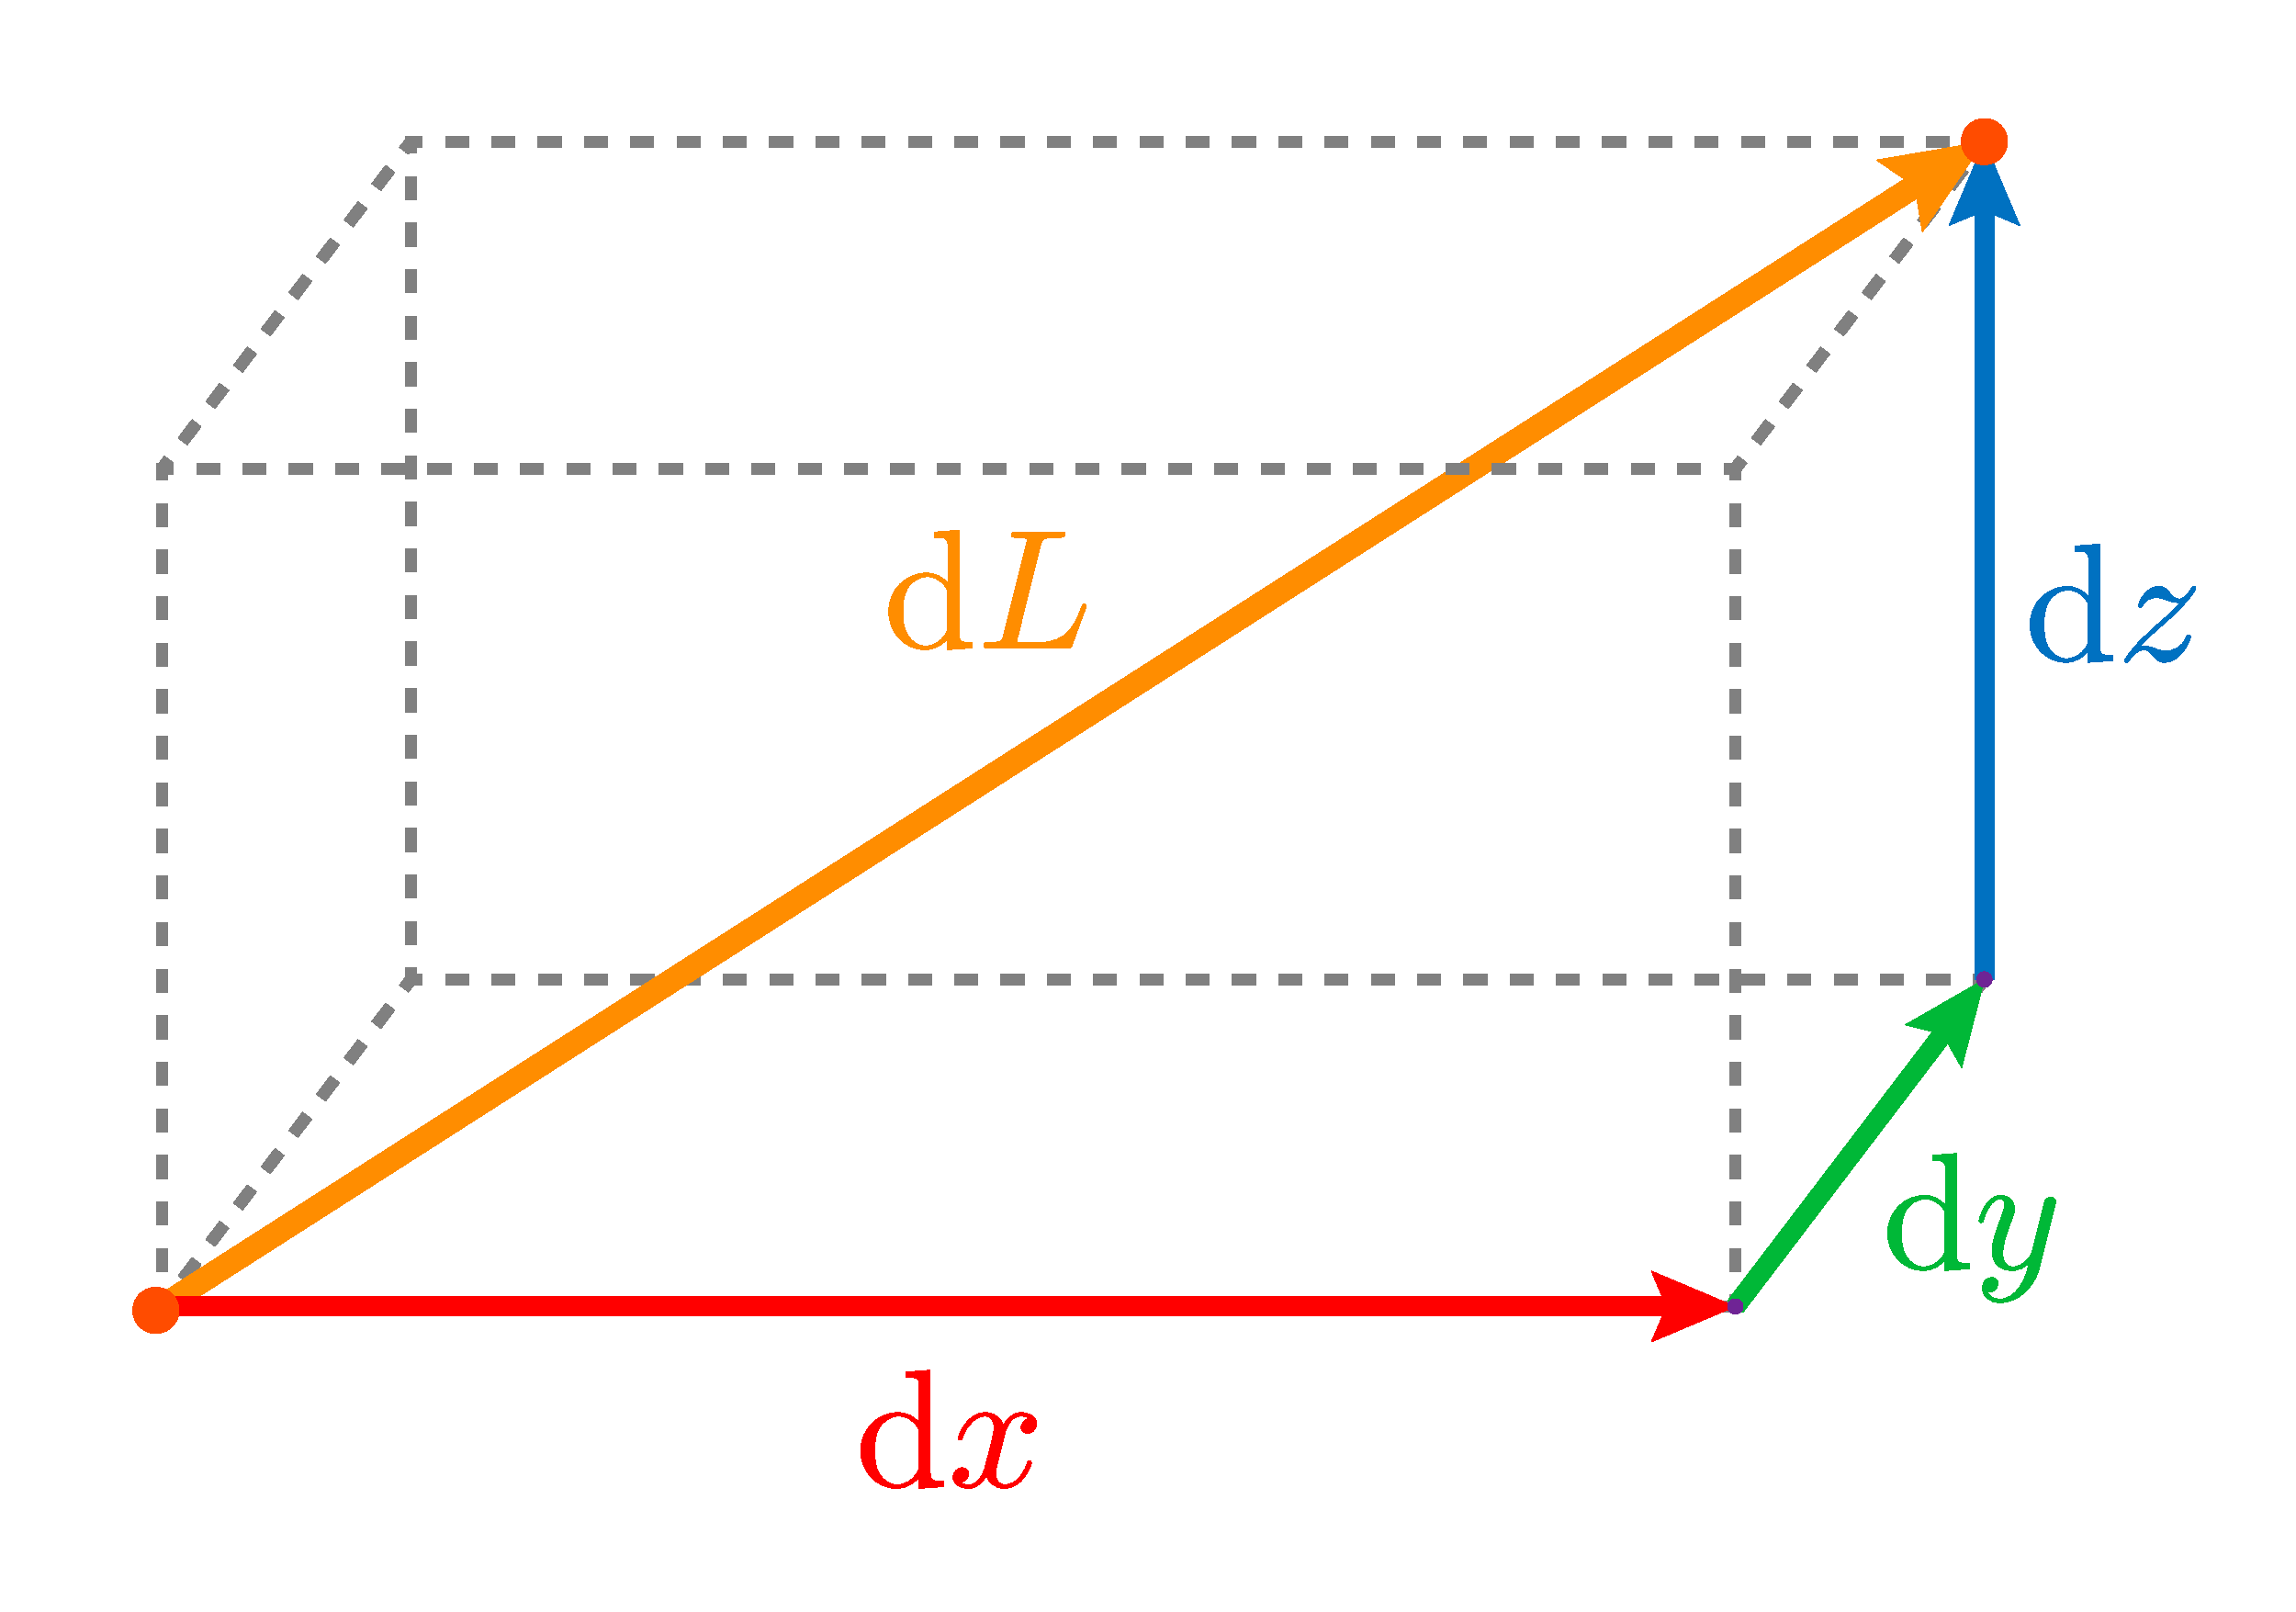
\includegraphics[width=0.32\textwidth]{diagrams/dL.pdf}
    \caption{$\dd{L}$ in terms of $\dd{x}$, $\dd{y}$, and $\dd{z}$} \label{fig:dL}
\end{wrapfigure}
However, what is $\dd{L}$? To find what $\dd{L}$ is, it is useful to think of it as a 3-dimensional vector. One important property of vectors is that they can be expressed as a sum of multiple vectors, and thus 3D vectors can be decomposed into their $x$, $y$, and $z$  components. Using this line of thinking, it can similarly be said that $\dd{L}$ can be
decomposed into the infinitesimals $\dd{x}$, $\dd{y}$, and $\dd{z}$, as visualized in Figure \ref{fig:dL}. Therefore, applying the 3D Pythagorean theorem:
\begin{equation*}
    \dd{L} = \sqrt{(\dd{x})^2+(\dd{y})^2+(\dd{z})^2}
\end{equation*}

However, this is not of much use, as $\dd{x}$, $\dd{y}$, and $\dd{z}$ are arbitrary. Thus, $\dd{t}$ is introduced into the equation by multiplying the equation by $\frac{\dd{t}}{\dd{t}}$, and with some algebraic manipulation, $\dd{L}$ can be expressed in terms of the derivatives of $x(t)$, $y(t)$, and $z(t)$ components of the curve, which can be easily evaluated \autocite{schlickerArcLength}:
\begin{equation*}
    \dd{L} = \sqrt{\frac{(\dd{x})^2+(\dd{y})^2+(\dd{z})^2}{(\dd{t})^2}} \cdot \dd{t} = \sqrt{\left(\dv{x}{t}\right)^2+\left(\dv{y}{t}\right)^2+\left(\dv{z}{t}\right)^2} \cdot \dd{t}
\end{equation*}
\bulletarrow Substituting in $x(t)$, $y(t)$, and $z(t)$:
\begin{align*}
    \Rightarrow \dd{L} & = \sqrt{\left(\dv{t}\left(\frac{\lambda}{2\pi S}Rt\cos{t}\right)\right)^2+\left(\dv{t}\left(\frac{\lambda}{2\pi S}Rt\sin{t}\right)\right)^2+\left(\dv{t}\left(\frac{\lambda}{2\pi S}Ht\right)\right)^2} \cdot \dd{t} \\
           &= \frac{\lambda}{2\pi S}\sqrt{\left(\dv{t}\left(Rt\cos{t}\right)\right)^2+\left(\dv{t}\left(Rt\sin{t}\right)\right)^2+\left(\dv{t}\left(Ht\right)\right)^2} \cdot \dd{t} \\
           &= \frac{\lambda}{2\pi S}\sqrt{(R\cos{t}-Rt\sin{t})^2+(R\sin{t}-Rt\cos{t})^2+H^2} \cdot \dd{t}
\end{align*}
\bulletarrow Expanding and simplifying:
\begin{align}
    \Rightarrow \dd{L} &= \frac{\lambda}{2\pi S}\sqrt{(R^2\cos^2{t}-\cancel{2R^2t\sin{t}\cos{t}}+R^2t^2\sin^2{t})+(R^2\sin^2{t}+\cancel{2R^2t\sin{t}\cos{t}}+R^2t^2\cos^2{t})+H^2} \cdot \dd{t} \notag \\ 
     &= \frac{\lambda}{2\pi S}\sqrt{R^2(\cancel{\sin^2{t} + \cos^2{t}})+ R^2t^2(\cancel{\sin^2{t}+\cos^2{t}})+H^2} \cdot \dd{t} \notag \\ 
     &= \frac{\lambda}{2\pi S}\sqrt{R^2 +H^2 + R^2t^2} \cdot \dd{t} \notag \\ 
     &= \frac{\lambda}{2\pi S}\sqrt{S^2 + R^2t^2} \cdot \dd{t} 
\end{align}
\bulletarrow Substituting this back into equation \ref{eq:arclen}, we finally obtain:
\begin{equation}
    L = \frac{\lambda}{2\pi S}\int_0^\frac{2\pi S}{\lambda} \sqrt{S^2 + R^2t^2} \cdot \dd{t} \label{eq:integral}
\end{equation}
